\section{Hours of Operation and Occupancy}
\label{sec:hoo}

\subsection{Hours of Operation}
\subsubsection{Overview}
Hours of operation are added to the model using operation start time and duration inputs. The start times and durations are assigned to each model through the sampling process using a set of distributions based on building type. They are then further broken down by weekday and weekend (Figure~\ref{fig:start_time} and Figure~\ref{fig:duration}). When applied to the model, the start time and duration establish the building's operating start and end times for weekdays and for weekends. Every schedule in the model is parametric (Section~\ref{sec:parametric_schedules}): a schedule is authored as a set of control points placed relative to the operating start and end times, so the sampled hours are not applied by stretching or shifting a fixed profile but by expanding each schedule around the building's own start and end times. Occupancy, lighting, plug loads, hot water draws, thermostat setbacks, and HVAC availability are all built from the same start and end times, which keeps them coordinated. Note that because the weekday and weekend start times and durations are sampled independently, they are not aligned in a given building model.

Some space uses keep their own clock regardless of the building's operating hours. A hotel guest room is occupied overnight when the front desk is quiet, and a hospital's nurses stations, patient rooms, emergency rooms, exam rooms, and kitchen operate around the clock. The schedule sets for these space types are flagged to ignore the building hours of operation and expand at their authored timing. Space types flagged as critical operation (data centers, operating rooms, patient rooms, emergency rooms, nurses stations, recovery rooms) additionally run their zone HVAC equipment continuously and count as always occupied for the purpose of air loop operation schedules.

\subsubsection{Hours of Operation Derivation}
We derived the hours of operation by applying the method introduced in \cite{bianchi2020modeling} to 1 year of AMI data from 6,070 buildings spread across eight utilities (the commercial schedules AMI data set). We first extracted the two-dimensional distribution of \textit{High Load Start Time} and \textit{High Load Duration} from this AMI data set, as an approximation of the schedule of hours of operations for each building type. Then, we compared this distribution with the inputs of ComStock at the start of
 the \href{https://www.nrel.gov/buildings/end-use-load-profiles.html}{End-Use Load Profiles} (EULP) calibration.

Figure~\ref{fig:utility_building_type} lists the number of buildings for each building type from each utility's AMI data set that was considered during the EULP project. The utility data sets and names are listed in Table 10 of the EULP Final Technical Report \citep{eulp_final_report}. Among the 15 building types considered in ComStock, 14 can be found in the commercial schedules AMI data set. The only exception is secondary schools, because all schools were grouped together in the AMI data.

We compared the distribution extracted from the commercial schedules AMI data set with the inputs of ComStock at the start of the EULP calibration. The results of the small office building type are presented in Figure~\ref{fig:small_office_season} to illustrate the process, because this building type has the largest sample size in the AMI data set. We considered two day types, working day vs. non-working day, and two season definitions---one defined by month, and the other defined by daily average outdoor air temperature. The distribution of hours of operation is more diffuse in the AMI data set than in the ComStock inputs at the start of EULP calibration. Also, the duration of high load is smaller in the real AMI data than in the previous ComStock assumptions.

We explored whether and how the hours of operation are influenced by season (in Figure~\ref{fig:small_office_season}) and by utility (in Figure \ref{fig:small_office_utility}). Some differences can be observed; however, due to the modeling complexity and the desire to create a nationally applicable approach that avoids overfitting to a specific utility region, we combined the AMI data across seasons and utilities to generate a distribution of hours of operation for each building type. These new distributions were applied to ComStock in place of the existing distributions.


\subsection{Occupancy}
\subsubsection{Occupancy Density}
Occupants are assigned to individual space types as an occupancy density (people/1000 ft\textsuperscript{2}). This value, when multiplied by the total zone floor area, determines the maximum number of people in a zone. Table~\ref{tab:occupancy_density_all} shows the occupancy densities for all space types included in ComStock.

Occupant density is a property of the space type and the template family, looked up through the space type's ASHRAE 62.1 ventilation category. For buildings whose templates are ASHRAE 90.1-2004 and later or DEER 2007 and later, the densities are the default occupant densities tabulated in ASHRAE Standard 62.1 for each ventilation category \citep{ashrae_62.1_2004}; where the standard tabulates no density for a category, the density of the corresponding prototype space type is used, and the data records which source applies. For the DOE Ref and earlier DEER templates, the densities are those of the reference building models of that era, which drew on ASHRAE Standard 62-1999 and the International Building Code 2003 \citep{icc_2003}. The building type definitions override a density only where a building type uses a space differently from the stock-wide record; the one such override in the current definitions is the hospital cafeteria, which is held at 10 people per 1,000 ft\textsuperscript{2} rather than the fast-food dining density of its ventilation category. Hotel guest rooms carry the ASHRAE 62.1 bedroom density of 10 people per 1,000 ft\textsuperscript{2}; the fraction of rooms that are occupied on a given night is represented through the guest room occupancy schedule rather than through separate occupied and vacant room space types.

\subsubsection{Occupancy Schedules}
\label{sec:parametric_schedules}
The maximum number of people in a zone (calculated from occupancy density and zone floor area) is multiplied by a fractional occupancy schedule with values ranging from zero to one to capture the variation in building occupancy throughout the day. Each space type carries a parametric schedule set that binds five schedules: occupancy, interior lighting, electric equipment, gas equipment, and hot water equipment. The occupancy schedule is the primary schedule of the set, and the four load schedules are derived from it, as described in Section~\ref{sec:derived_schedules}.

An occupancy schedule is authored as a short list of control points rather than as a fixed hourly profile. Each control point is a time, stated relative to the operating start time (\emph{st}) or end time (\emph{et})---\emph{st-1}, \emph{st}, \emph{et-1}, \emph{et+6}---and a value, stated as the schedule's base fraction, its peak fraction, or a fraction of the range between them. A separate list of control points is authored for weekdays, Saturdays, and Sundays and holidays, and for the summer and winter design days. Each schedule also carries standalone start and end times, which are used when the building supplies no hours of operation. When the model is built, the building's sampled weekday and weekend start and end times replace the standalone times, and the control points are expanded to a 15-minute profile by smooth interpolation between consecutive points, held flat from midnight to the first point and from the last point to midnight. Figure~\ref{fig:parametric_control_points} illustrates the expansion of a four-point profile. A space type whose set is flagged to keep its own clock expands at its authored times instead.

The control points were fitted to source schedules rather than authored from scratch, and each schedule set records the provenance of its occupancy profile. Most profiles were fitted to the occupancy schedules in the Pacific Northwest National Laboratory building energy standards support data, which underlie the ASHRAE 90.1 prototype buildings, or to the occupancy schedules of the ComStock prototype space types that preceded them, several of which were themselves derived from end-use data during the EULP project. A smaller number are the legacy prototype profiles carried over directly, and a few---hotel guest rooms and dwelling units, whose occupancy is highest overnight---were authored by hand. Figures~\ref{fig:parametric_occupancy_1} and~\ref{fig:parametric_occupancy_2} show the weekday occupancy profiles of the space types that make up most of the stock's floor area, expanded at each schedule's standalone hours. Table~\ref{tab:parametric_schedule_sets} lists the schedule set of every space type with its standalone hours, base and peak fractions, number of control points, and provenance.

Occupancy schedules in ComStock buildings are further adjusted so that the total daily occupancy in the building stock does not exceed the average daily occupancy of the United States building stock as derived from analysis of locations in the American Time Use Survey \citep{atus2018} Activity file. This adjustment applies a 23\% reduction factor to all occupant schedule values, resulting in a peak daily total occupancy in ComStock models of approximately 115M people.

\subsubsection{Occupancy Activity Schedules}
Occupancy activity schedules represent the total heat gain per person, including convective, radiant, and latent heat. An internal EnergyPlus algorithm determines the fraction of the total load that is sensible and latent. The sensible portion is further divided into radiant and convective using the default fraction radiant value. ComStock uses a constant activity level of 120 watts per person in every space type, in every state.

\pagebreak

\begin{figure}
   \centering \includegraphics[width=1\textwidth]{figures/start_time.png}
   \caption{Operating hours' start time distributions.}
    \label{fig:start_time}
\end{figure}

\begin{figure}
    \centering \includegraphics[width=1\textwidth]{figures/duration.png}
    \caption{Operating hours' duration distributions.}
    \label{fig:duration}
\end{figure}

\begin{figure}
    \centering 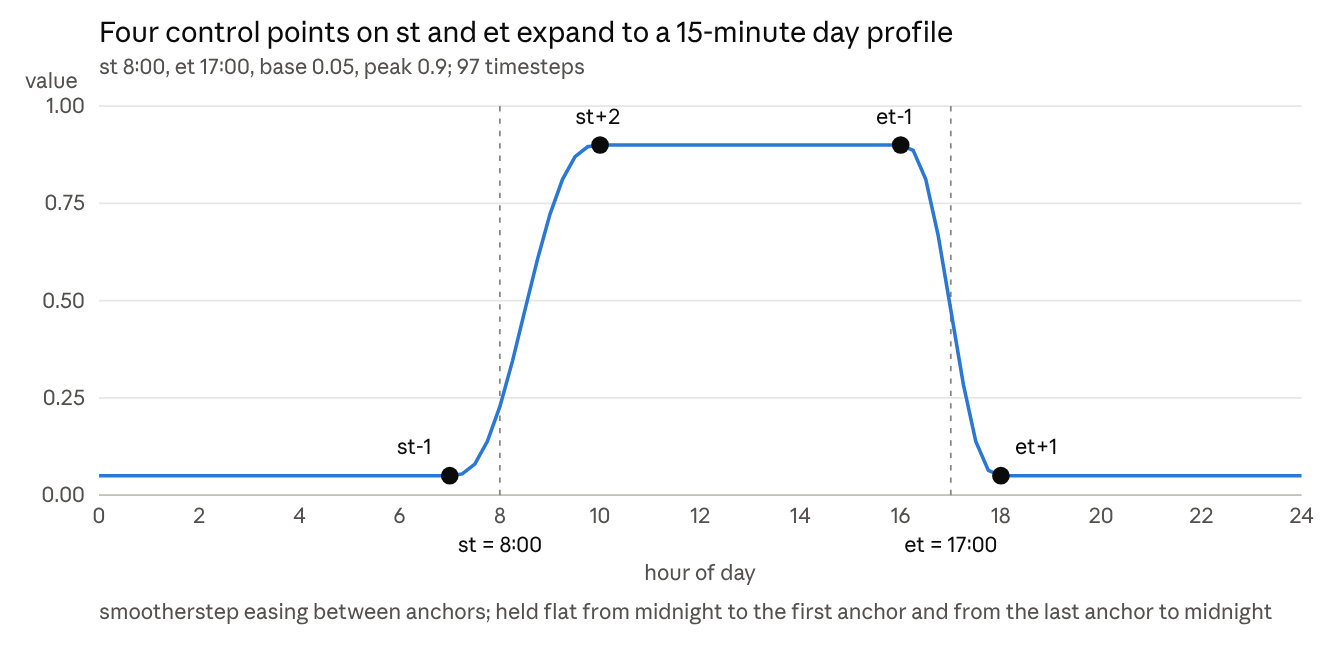
\includegraphics[width=0.9\textwidth]{figures/parametric_control_points.png}
    \caption[Expansion of a parametric schedule from control points]{Expansion of a parametric schedule from four control points placed relative to the operating start time (st) and end time (et). The sampled hours of operation set st and et; the control points are then interpolated to a 15-minute profile and held flat outside the first and last points.}
    \label{fig:parametric_control_points}
\end{figure}

\begin{figure}
    \centering 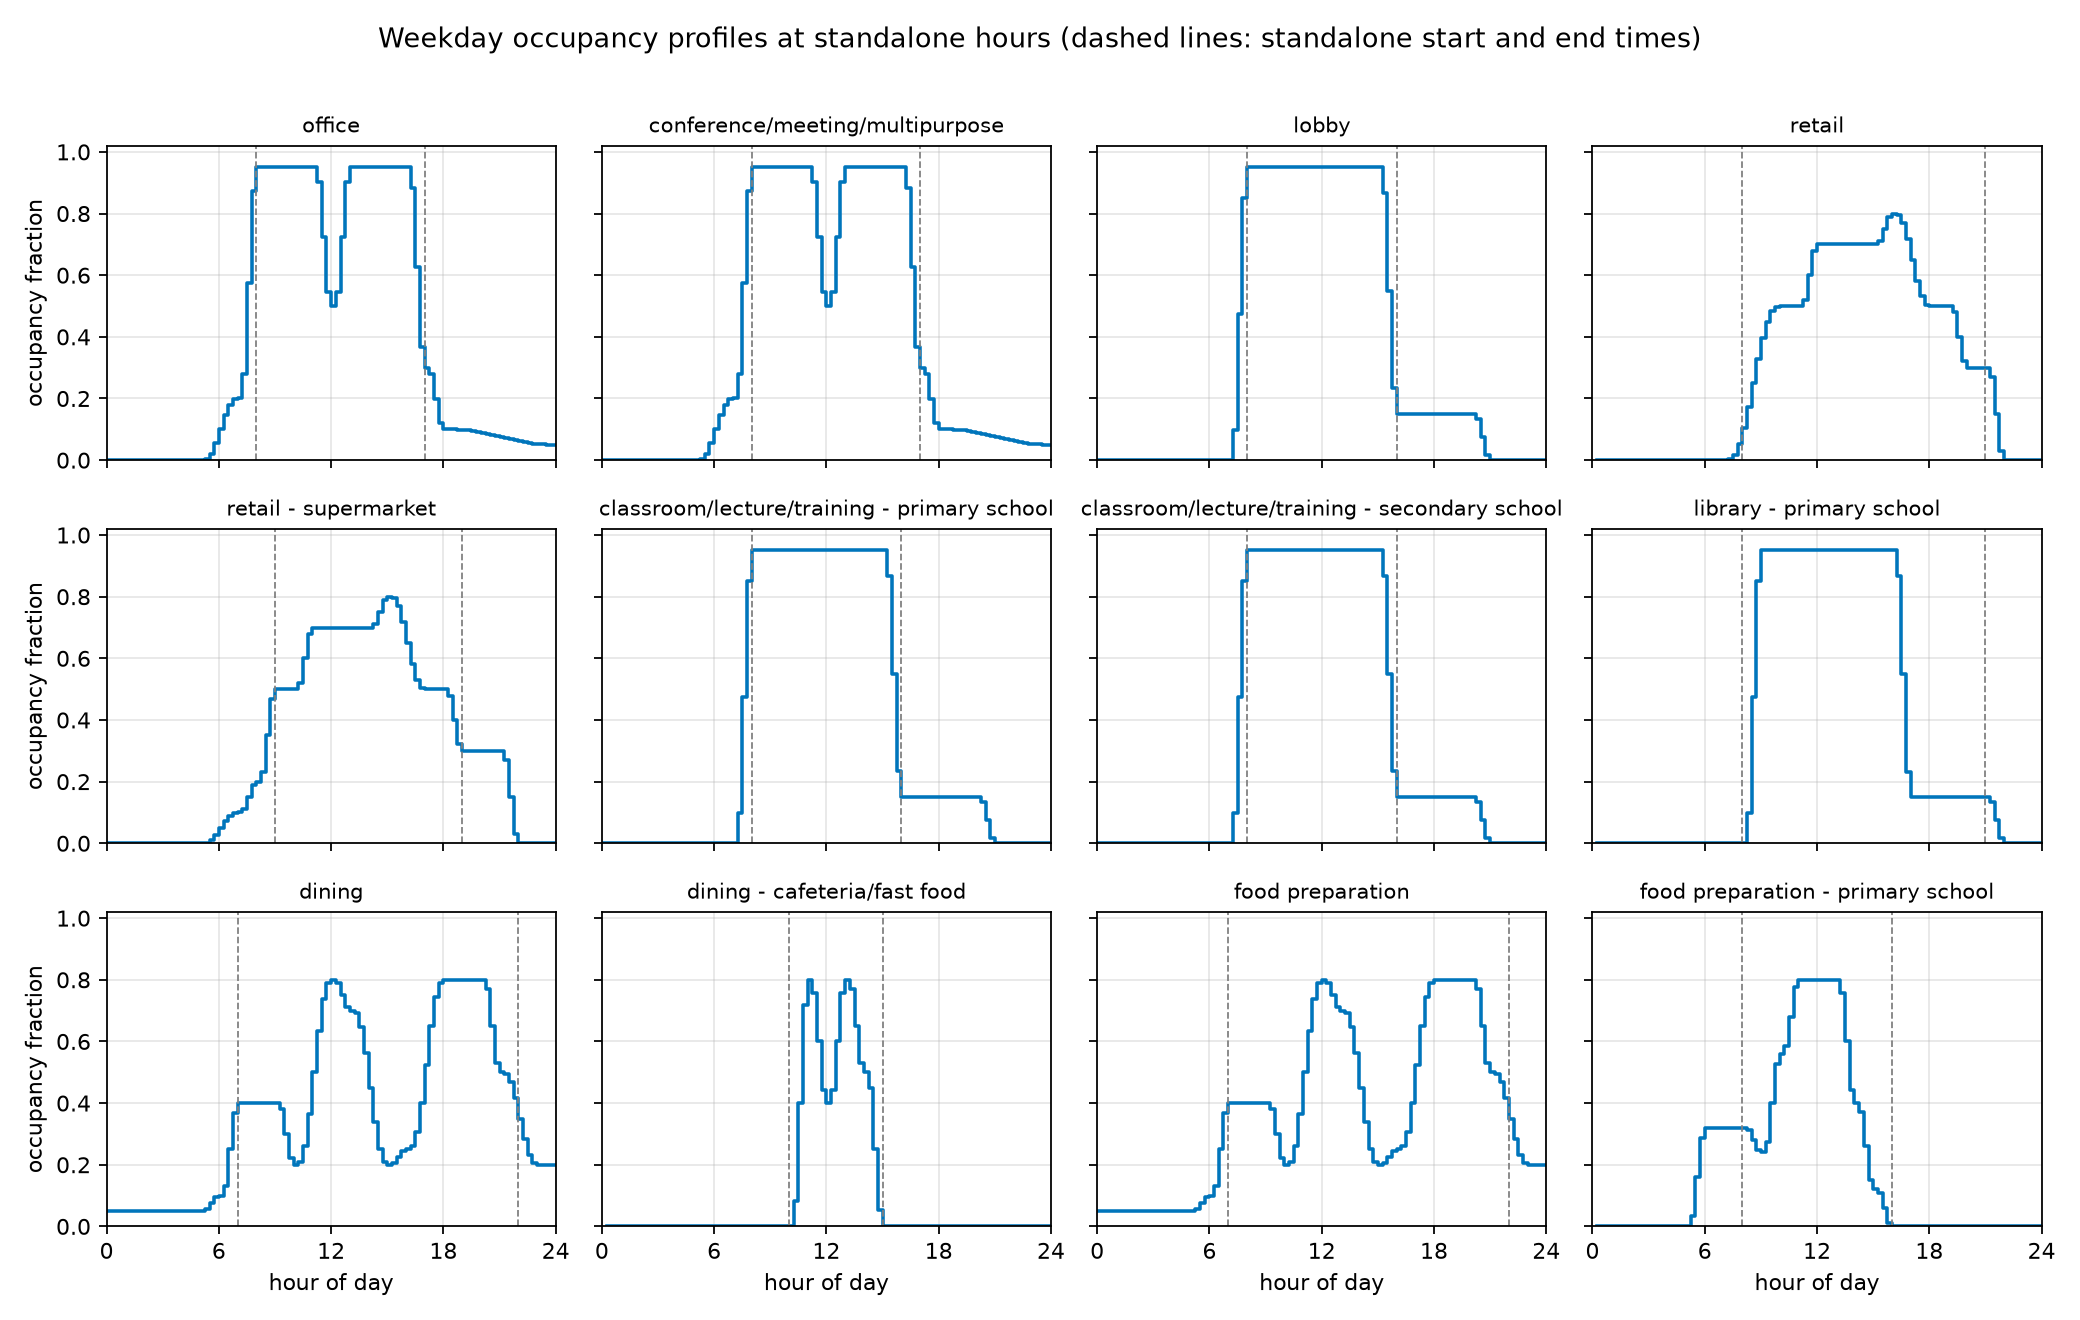
\includegraphics[width=1\textwidth]{figures/parametric_occupancy_1.png}
    \caption[Parametric weekday occupancy profiles, part 1]{Weekday occupancy profiles of office, retail, education, and food service space types, expanded at each schedule's standalone start and end times. In a model, the building's sampled hours of operation replace the standalone times.}
    \label{fig:parametric_occupancy_1}
\end{figure}

\begin{figure}
    \centering 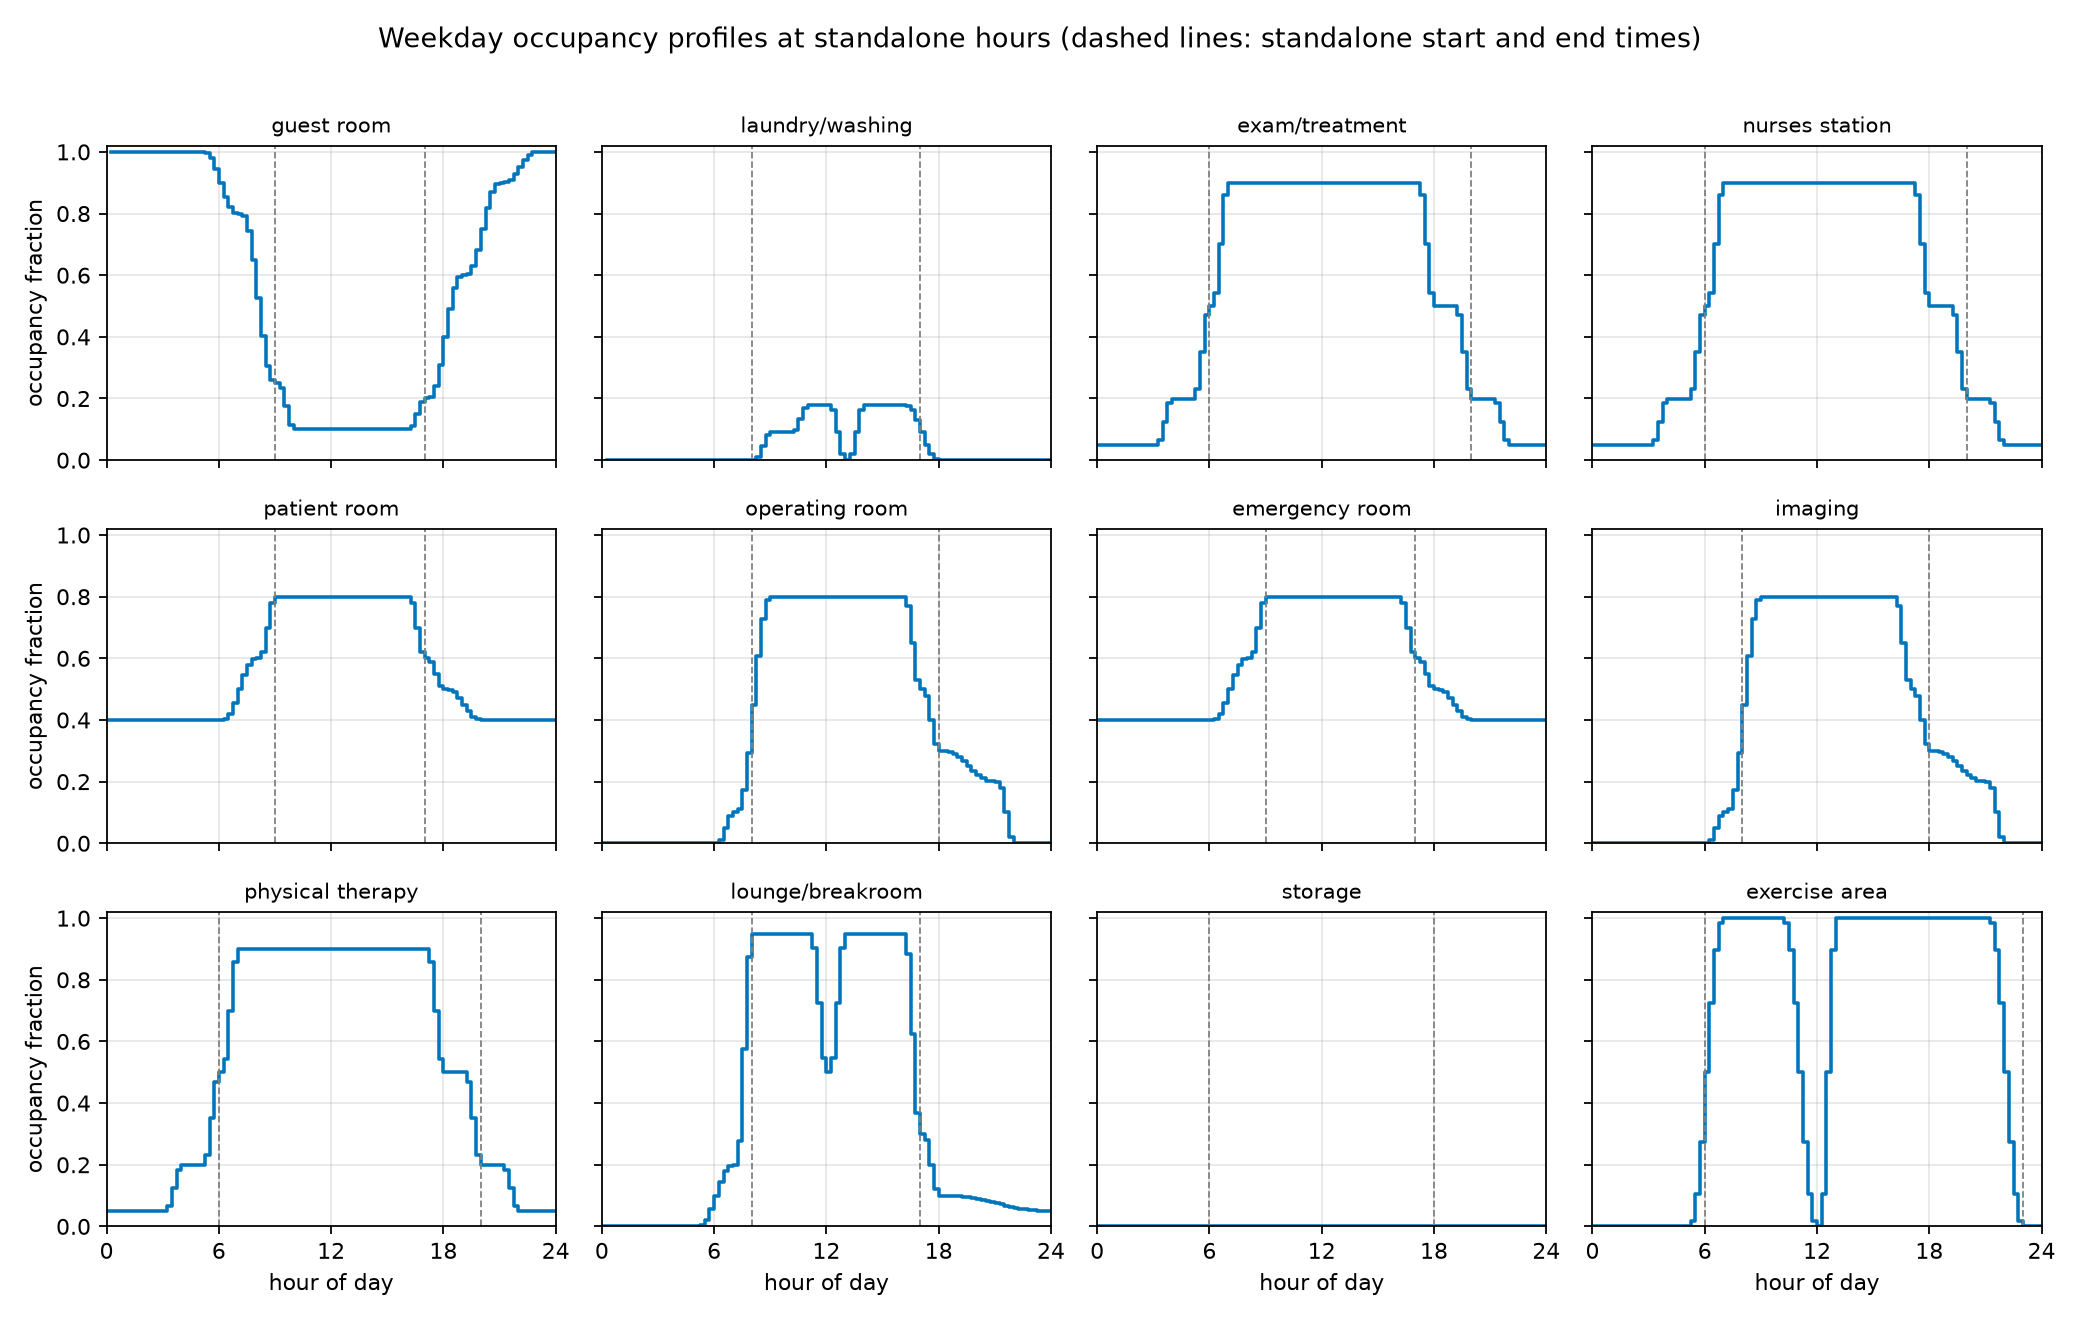
\includegraphics[width=1\textwidth]{figures/parametric_occupancy_2.png}
    \caption[Parametric weekday occupancy profiles, part 2]{Weekday occupancy profiles of lodging, healthcare, warehouse, and support space types, expanded at each schedule's standalone start and end times. Guest rooms and the hospital patient care space types keep their authored timing regardless of the building's hours of operation.}
    \label{fig:parametric_occupancy_2}
\end{figure}
